
%(BEGIN_QUESTION)
% Copyright 2010, Tony R. Kuphaldt, released under the Creative Commons Attribution License (v 1.0)
% This means you may do almost anything with this work of mine, so long as you give me proper credit

Sketch the wires necessary to connect a solid-state proximity switch to input channel {\tt Ix.8} of a Siemens SM 321 discrete input card (model 6ES7321-1BP00-0AA0).  The internal schematic diagram of the first channel ({\tt Ix.0}) is shown as ``typical'' for all the channels:

$$\includegraphics[width=15.5cm]{i04544x01.eps}$$

Also, identify whether this is a {\it sinking} or a {\it sourcing} proximity switch, and sketch the directions of all currents through your sketched wires.

\vfil 

\underbar{file i04544}
\eject
%(END_QUESTION)





%(BEGIN_ANSWER)

This is a graded question -- no answers or hints given!

%(END_ANSWER)





%(BEGIN_NOTES)

This particular proximity switch {\it sinks} current from the input module (arrows drawn in the direction of conventional flow):

$$\includegraphics[width=15.5cm]{i04544x02.eps}$$

Note that the PLC input card has the ability to either source or sink current at each input, owing to the full-wave bridge rectifier which guarantees the optocoupler's LED will receive current in the correct direction no matter how current may enter or exit the input terminal.

%INDEX% PLC, I/O: discrete I/O device wiring

%(END_NOTES)


